\documentclass[a4paper, titlepage]{article}

% For equations
\usepackage{amsmath}

% For including figures
\usepackage{graphicx}
\usepackage{float}

% Bibiliography setup
\usepackage[square]{natbib}
\bibliographystyle{agsm}
\usepackage[nottoc]{tocbibind}

% For typesetting matlab
\usepackage{listings}
\usepackage{color} %red, green, blue, yellow, cyan, magenta, black, white
\definecolor{mygreen}{RGB}{28,172,0} % color values Red, Green, Blue
\definecolor{mylilas}{RGB}{170,55,241}

\lstset{language=Matlab,%
    basicstyle=\small,
    breaklines=true,%
    frame = single,
    morekeywords={matlab2tikz},
    keywordstyle=\color{blue},%
    morekeywords=[2]{1}, keywordstyle=[2]{\color{black}},
    identifierstyle=\color{black},%
    stringstyle=\color{mylilas},
    commentstyle=\color{mygreen},%
    showstringspaces=false,
    numbers=left,%
    numberstyle={\tiny \color{black}},% size of the numbers
    numbersep=9pt, % this defines how far the numbers are from the text
    emph=[1]{for,end,break},emphstyle=[1]\color{red}, %some words to emphasise
    %emph=[2]{word1,word2}, emphstyle=[2]{style},    
}


%\title{Assignment 3\\
%System description and analysis\\
%\large EEA004}
%\author{Dan Thilderkvist, Philip Gutierrez}

\begin{document}

%\maketitle

\begin{titlepage}
  \begin{center}
    \vspace*{1cm}
    
\includegraphics[scale=1.0]{../figures/hig_logo_eng.png}\\
    \vspace{1.5cm}
    \large EEA004 - Multivariable and Nonlinear Control Systems\\
    \large Assignment 3\\
    \vspace{1.5cm}
    Group 4\\
    Dan Thilderkvist and Philip Gutierrez\\
    dan.thilderkvist@hotmail.com philipgutierrez67@gmail.com\\
    Files: main.m\\
    
    \vspace{1cm}
    \today
  \end{center}
\end{titlepage}

\tableofcontents
\clearpage



\section{Introduction}

This assignment is a continuation of the previous two assignments where an air handler is analyzed.
Here we will look closer at two of the non-linear components of the system, namely the heater and the valve that controls it.
Both the heater and the valve have non-linear, but complementary, characteristics which compensate for each other.  However, the valve also exhibits valve authority effect which compromises the compensation between heater and valve.  These non-linearities will be analyzed closer. 
\citep[p.123]{glad00}

\subsection{Theory}
\section{Method}
\subsection{System Transfer Function}
The system to be analyzed is provided and is specified to be:

\begin{equation}
	G(s) = \frac{1}{(s^2+s+1)(s+3)}
	\label{equ:system}
\end{equation}

The system will be controlled by a valve which is considered to be static.  This valve has a gain $K_vs$, known as the "valve coefficient", and is available only with specific values.
With the addition of the gain $K_vs$ the new dynamic system becomes:

\begin{equation}
	G_{kv}(s) = \frac{K_{vs}}{(s^2+s+1)(s+3)} for K_{vs}=1, 1.6, 2.5, 4, 6.3, 10, and 16.
	\label{equ:systemTF}
\end{equation}


\subsection{Circle Criteria}

The method of Circle Criteria will be used to identify the valve with maximum power.  The exact nonlinearity is not known, but it is known to be limited to be inside the region specified by the blue arches as seen in figure \ref{fig:valvepower}.

\begin{figure}[h!]
\center
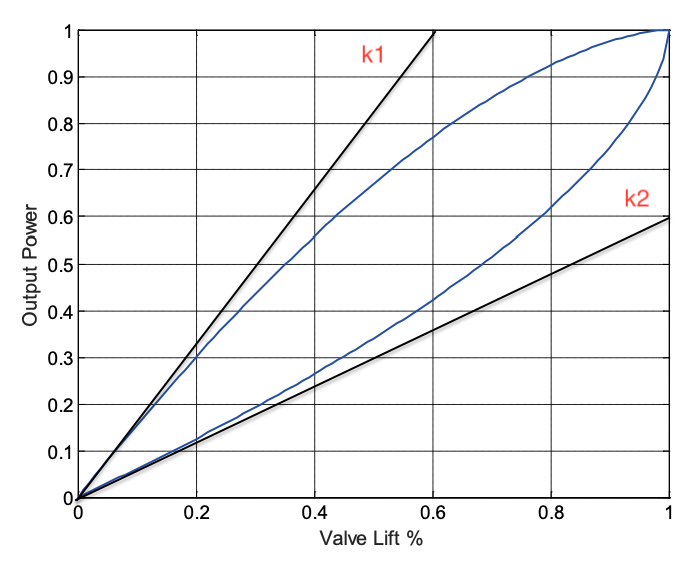
\includegraphics[scale=0.25]{../figures/valveOutputPower.png}
\caption{Valve Output Power}
\label{fig:valvepower}
\end{figure}

To apply the circle criteria, the region of known nonlinearity is bounded by two lines with slopes $k_{1}$ and $k_{2}$.  By inspection, these slopes are chosen to bound a region that includes the known region of nonlinearity of the valves.  From figure \ref{fig:valvepower} we find that:

\begin{equation}
k_{1} = \frac{1-0}{0.6-0} = \frac{1}{0.6}
\label{equ:k1_value}
\end{equation}

\begin{equation}
k_{2} = \frac{0.6-0}{1-0} = 0.6
\label{equ:k2_value}
\end{equation}

The values of $k_{1}$ and $k_{2}$ are used to form an exclusion region in the Nyquist diagram bounded by a circle which intersects the real axis at 1/$k_{1}$ and 1/$k_{2}$.  See Nyquist diagrams in the results section.

\section{Results}

The following Nyquist diagrams include a circle of exclusion which is bounded by $1/k_{1}$ and $1/k_{2}$.  The diagrams also include an exclusion region bounded by $1/k_{2}$ (shown as a vertical line in the graphs) which is used when analyzing the case with saturation in the valve.

\begin{figure}[h!]
\center
\includegraphics[scale=0.25]{../code/figures/nyquist1.png}
\caption{Nyquist diagram for $K_{vs}=1.0$}
\label{fig:nyquist1}
\end{figure}

\begin{figure}[h!]
\center
\includegraphics[scale=0.25]{../code/figures/nyquist2.png}
\caption{Nyquist diagram for $K_{vs}=1.6$}
\label{fig:nyquist2}
\end{figure}

\begin{figure}[h!]
\center
\includegraphics[scale=0.25]{../code/figures/nyquist3.png}
\caption{Nyquist diagram for $K_{vs}=2.5$}
\label{fig:nyquist3}
\end{figure}

\begin{figure}[h!]
\center
\includegraphics[scale=0.25]{../code/figures/nyquist4.png}
\caption{Nyquist diagram for $K_{vs}=4.0$}
\label{fig:nyquist4}
\end{figure}

\begin{figure}[h!]
\center
\includegraphics[scale=0.25]{../code/figures/nyquist5.png}
\caption{Nyquist diagram for $K_{vs}=6.3$}
\label{fig:nyquist5}
\end{figure}

\begin{figure}[h!]
\center
\includegraphics[scale=0.25]{../code/figures/nyquist6.png}
\caption{Nyquist diagram for $K_{vs}=10$}
\label{fig:nyquist6}
\end{figure}

\begin{figure}[h!]
\center
\includegraphics[scale=0.25]{../code/figures/nyquist7.png}
\caption{Nyquist diagram for $K_{vs}=16$}
\label{fig:nyquist7}
\end{figure}


\section{Discussion}
\section{Conclusion}




\clearpage
\bibliography{reference}

\clearpage
\appendix

\section{Appendix}
Here is the Matlab code used to generate the results in the report and the figures.

\lstinputlisting{../code/main.m}

\end{document}